
\documentclass{article}
\usepackage{graphicx}
\usepackage{float}
\usepackage{hyperref}
\usepackage{geometry}
\geometry{a4paper, margin=1in}

\title{Weather Progression: April 2, 2020}
\author{Weather Analysis System}
\date{\today}

\begin{document}
\maketitle

\section{Analysis Overview}
This analysis shows the progression of weather conditions across nine regional airports throughout April 2, 2020. The maps are shown at four key times during the day: midnight (00:00), early morning (06:00), noon (12:00), and evening (18:00).

\subsection{Airports Included}
\begin{itemize}
    \item \textbf{KRZL}: Reedsburg Municipal
    \item \textbf{KRYV}: Watertown Municipal
    \item \textbf{KMKE}: Milwaukee
    \item \textbf{KRPJ}: Rochelle Municipal
    \item \textbf{KORD}: Chicago O'Hare
    \item \textbf{KJOT}: Joliet Regional
    \item \textbf{KPNT}: Pontiac Municipal
    \item \textbf{KOXI}: Starke County
    \item \textbf{KIGQ}: Boone County
\end{itemize}

\subsection{Weather Information Displayed}
\begin{itemize}
    \item Temperature (airport marker color scales with temperature)
    \item Sky Condition (color-coded boxes)
    \item Wind Speed and Direction (blue arrows)
    \item Ceiling Height
\end{itemize}

\section{Weather Progression}

\begin{figure}[H]
    \centering
    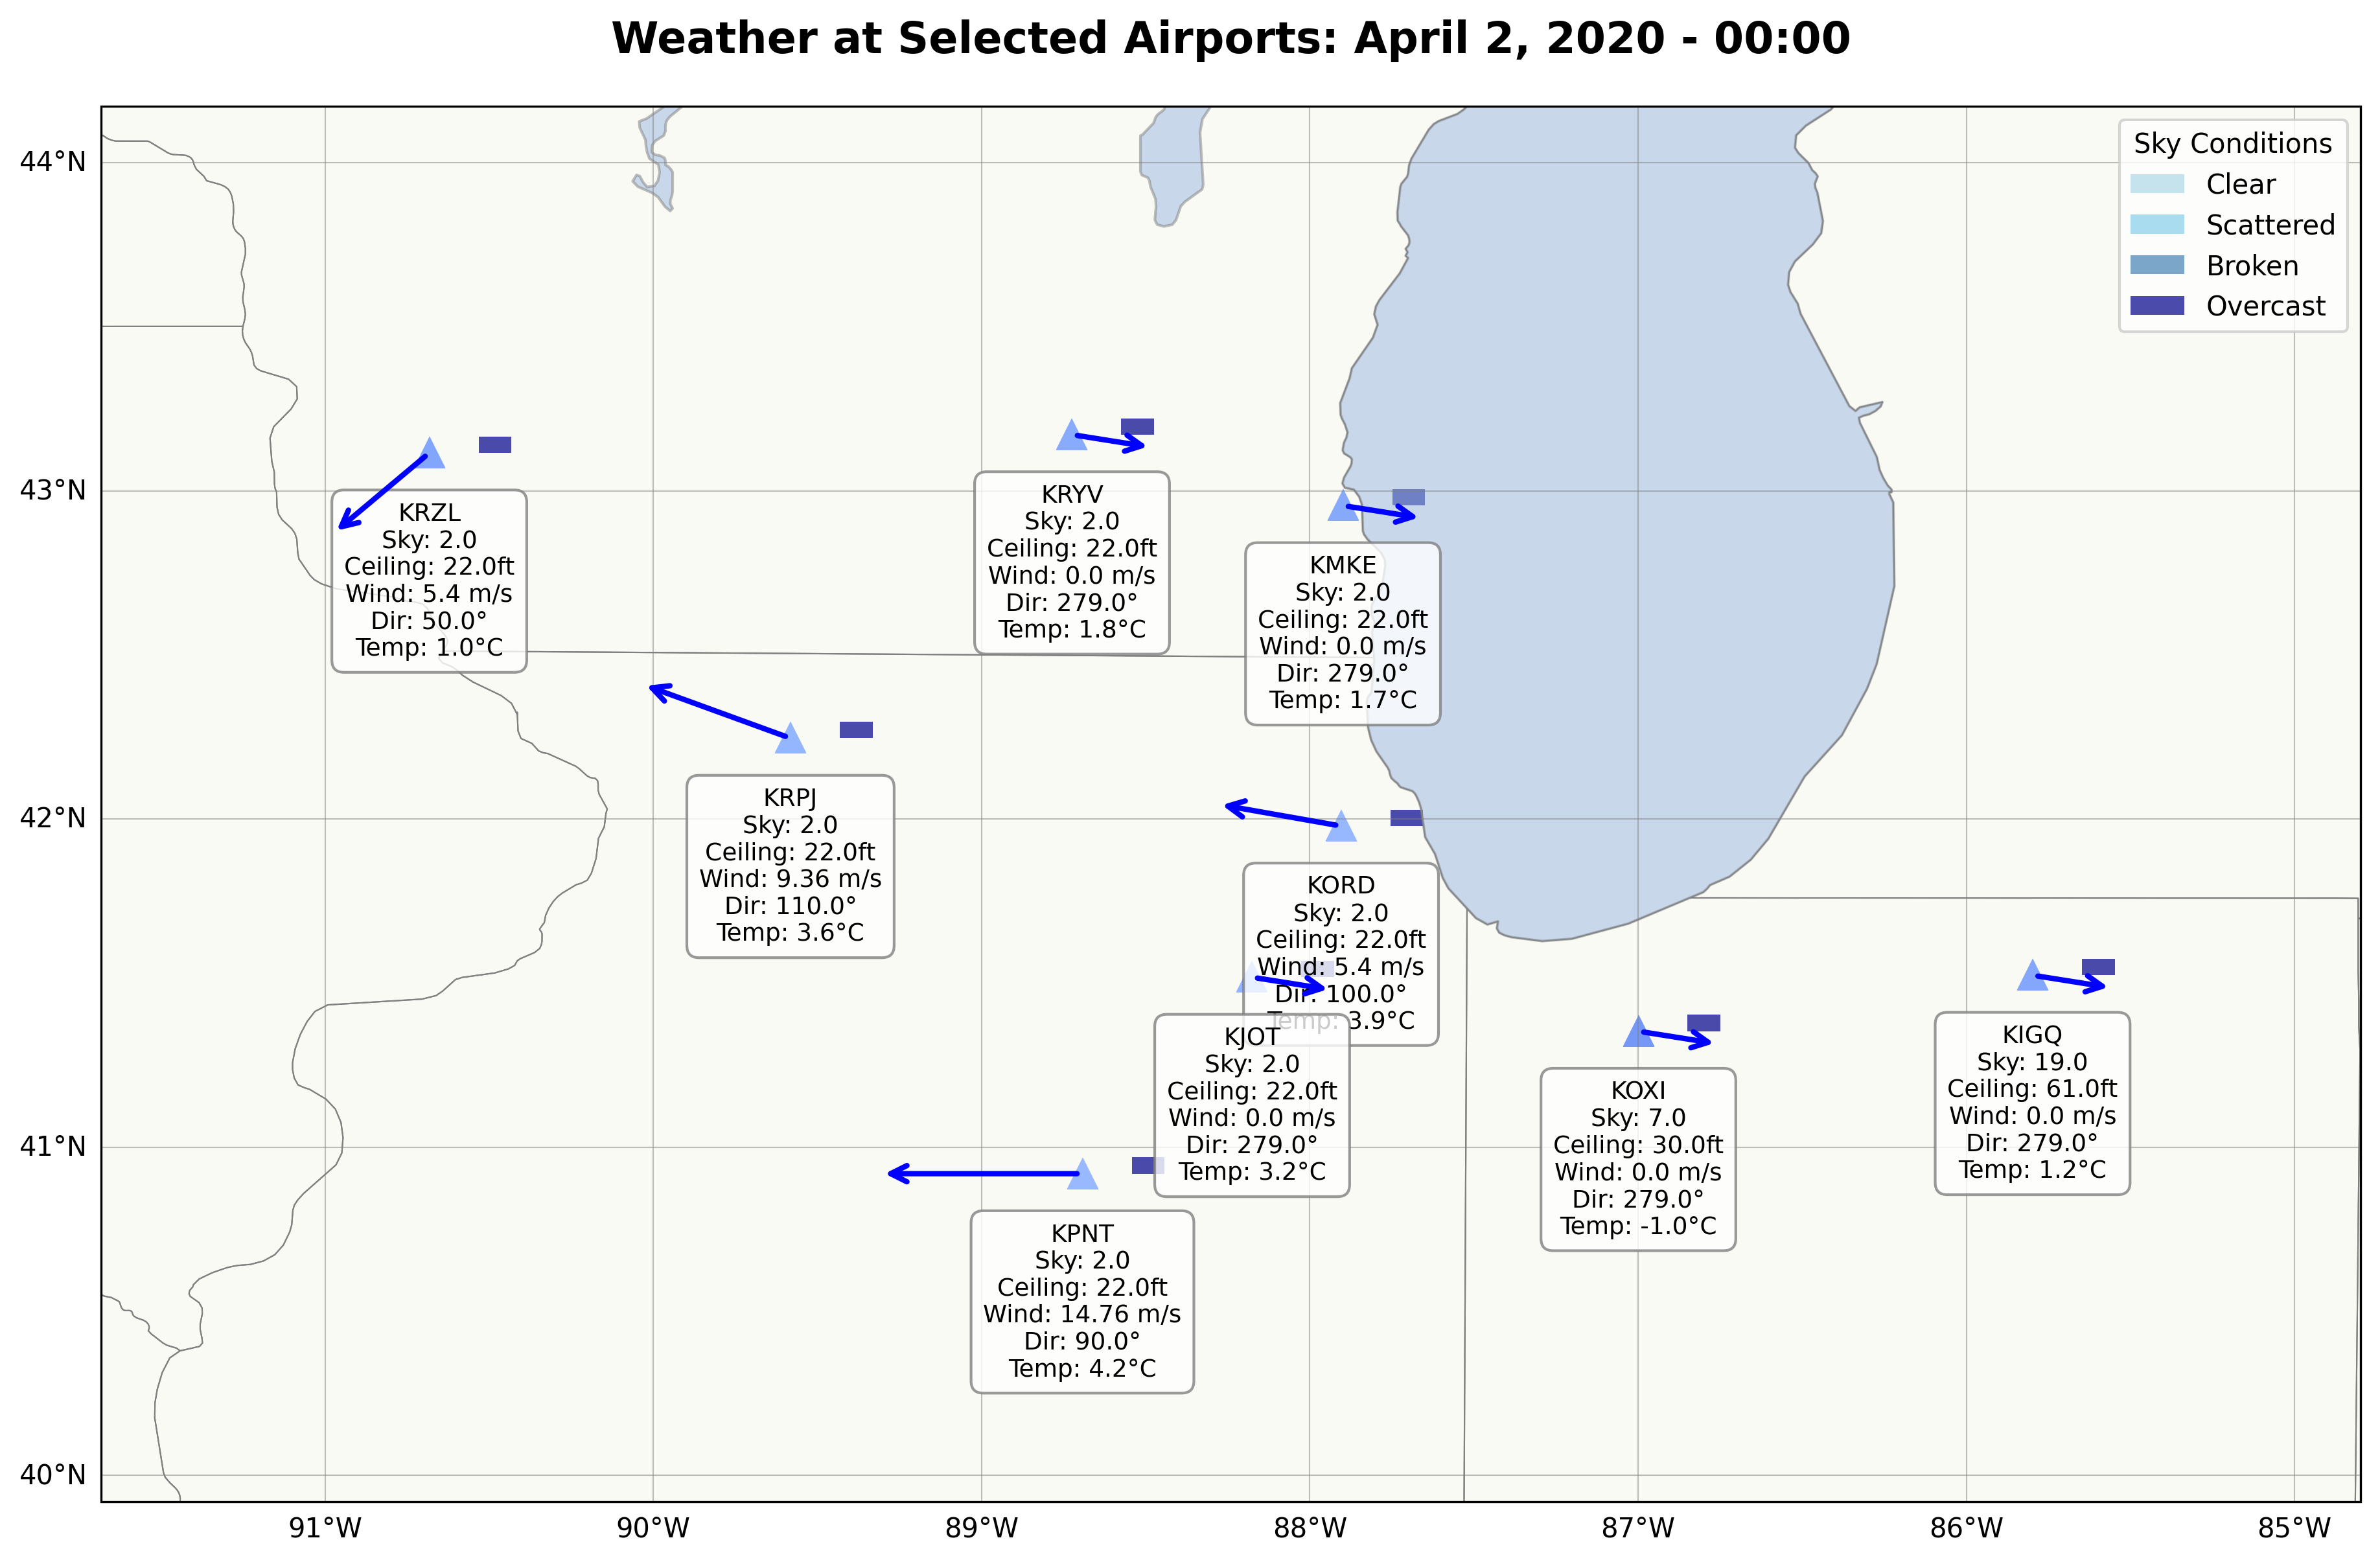
\includegraphics[width=\textwidth]{weather_map_00_00.png}
    \caption{Weather at Selected Airports: April 2, 2020 - 00:00}
    \label{fig:weather_00_00}
\end{figure}

\begin{figure}[H]
    \centering
    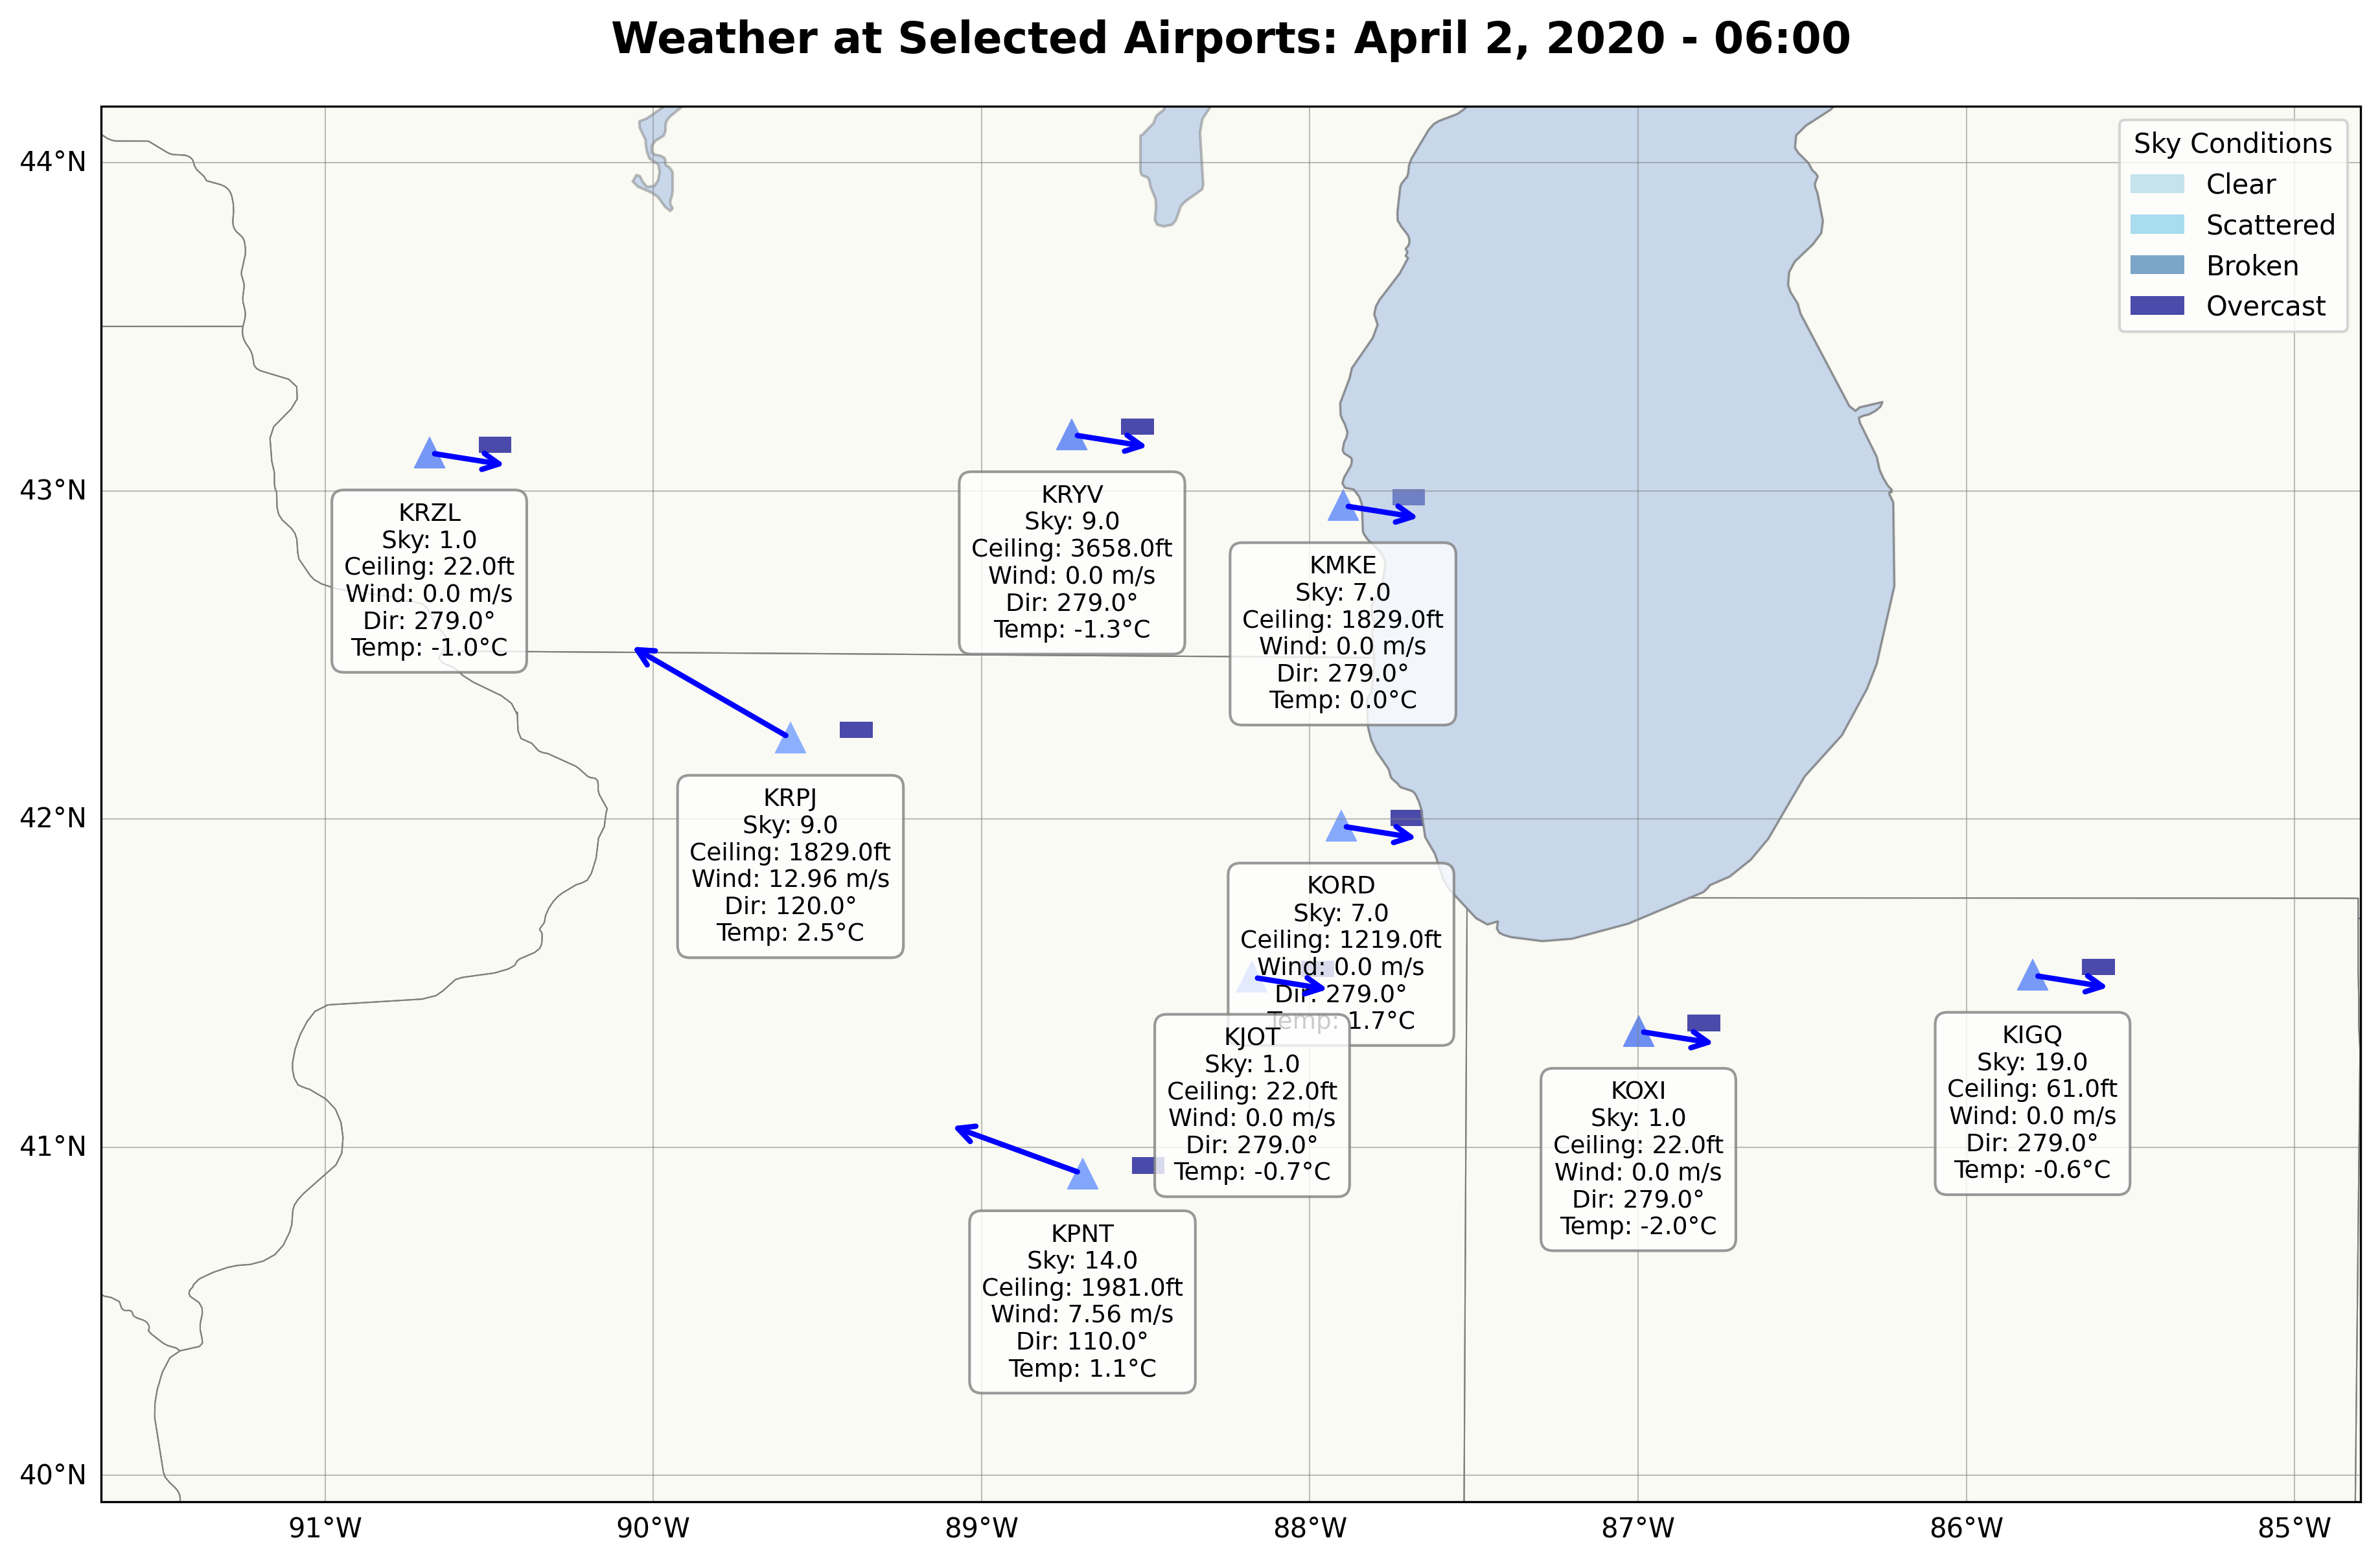
\includegraphics[width=\textwidth]{weather_map_06_00.png}
    \caption{Weather at Selected Airports: April 2, 2020 - 06:00}
    \label{fig:weather_06_00}
\end{figure}

\begin{figure}[H]
    \centering
    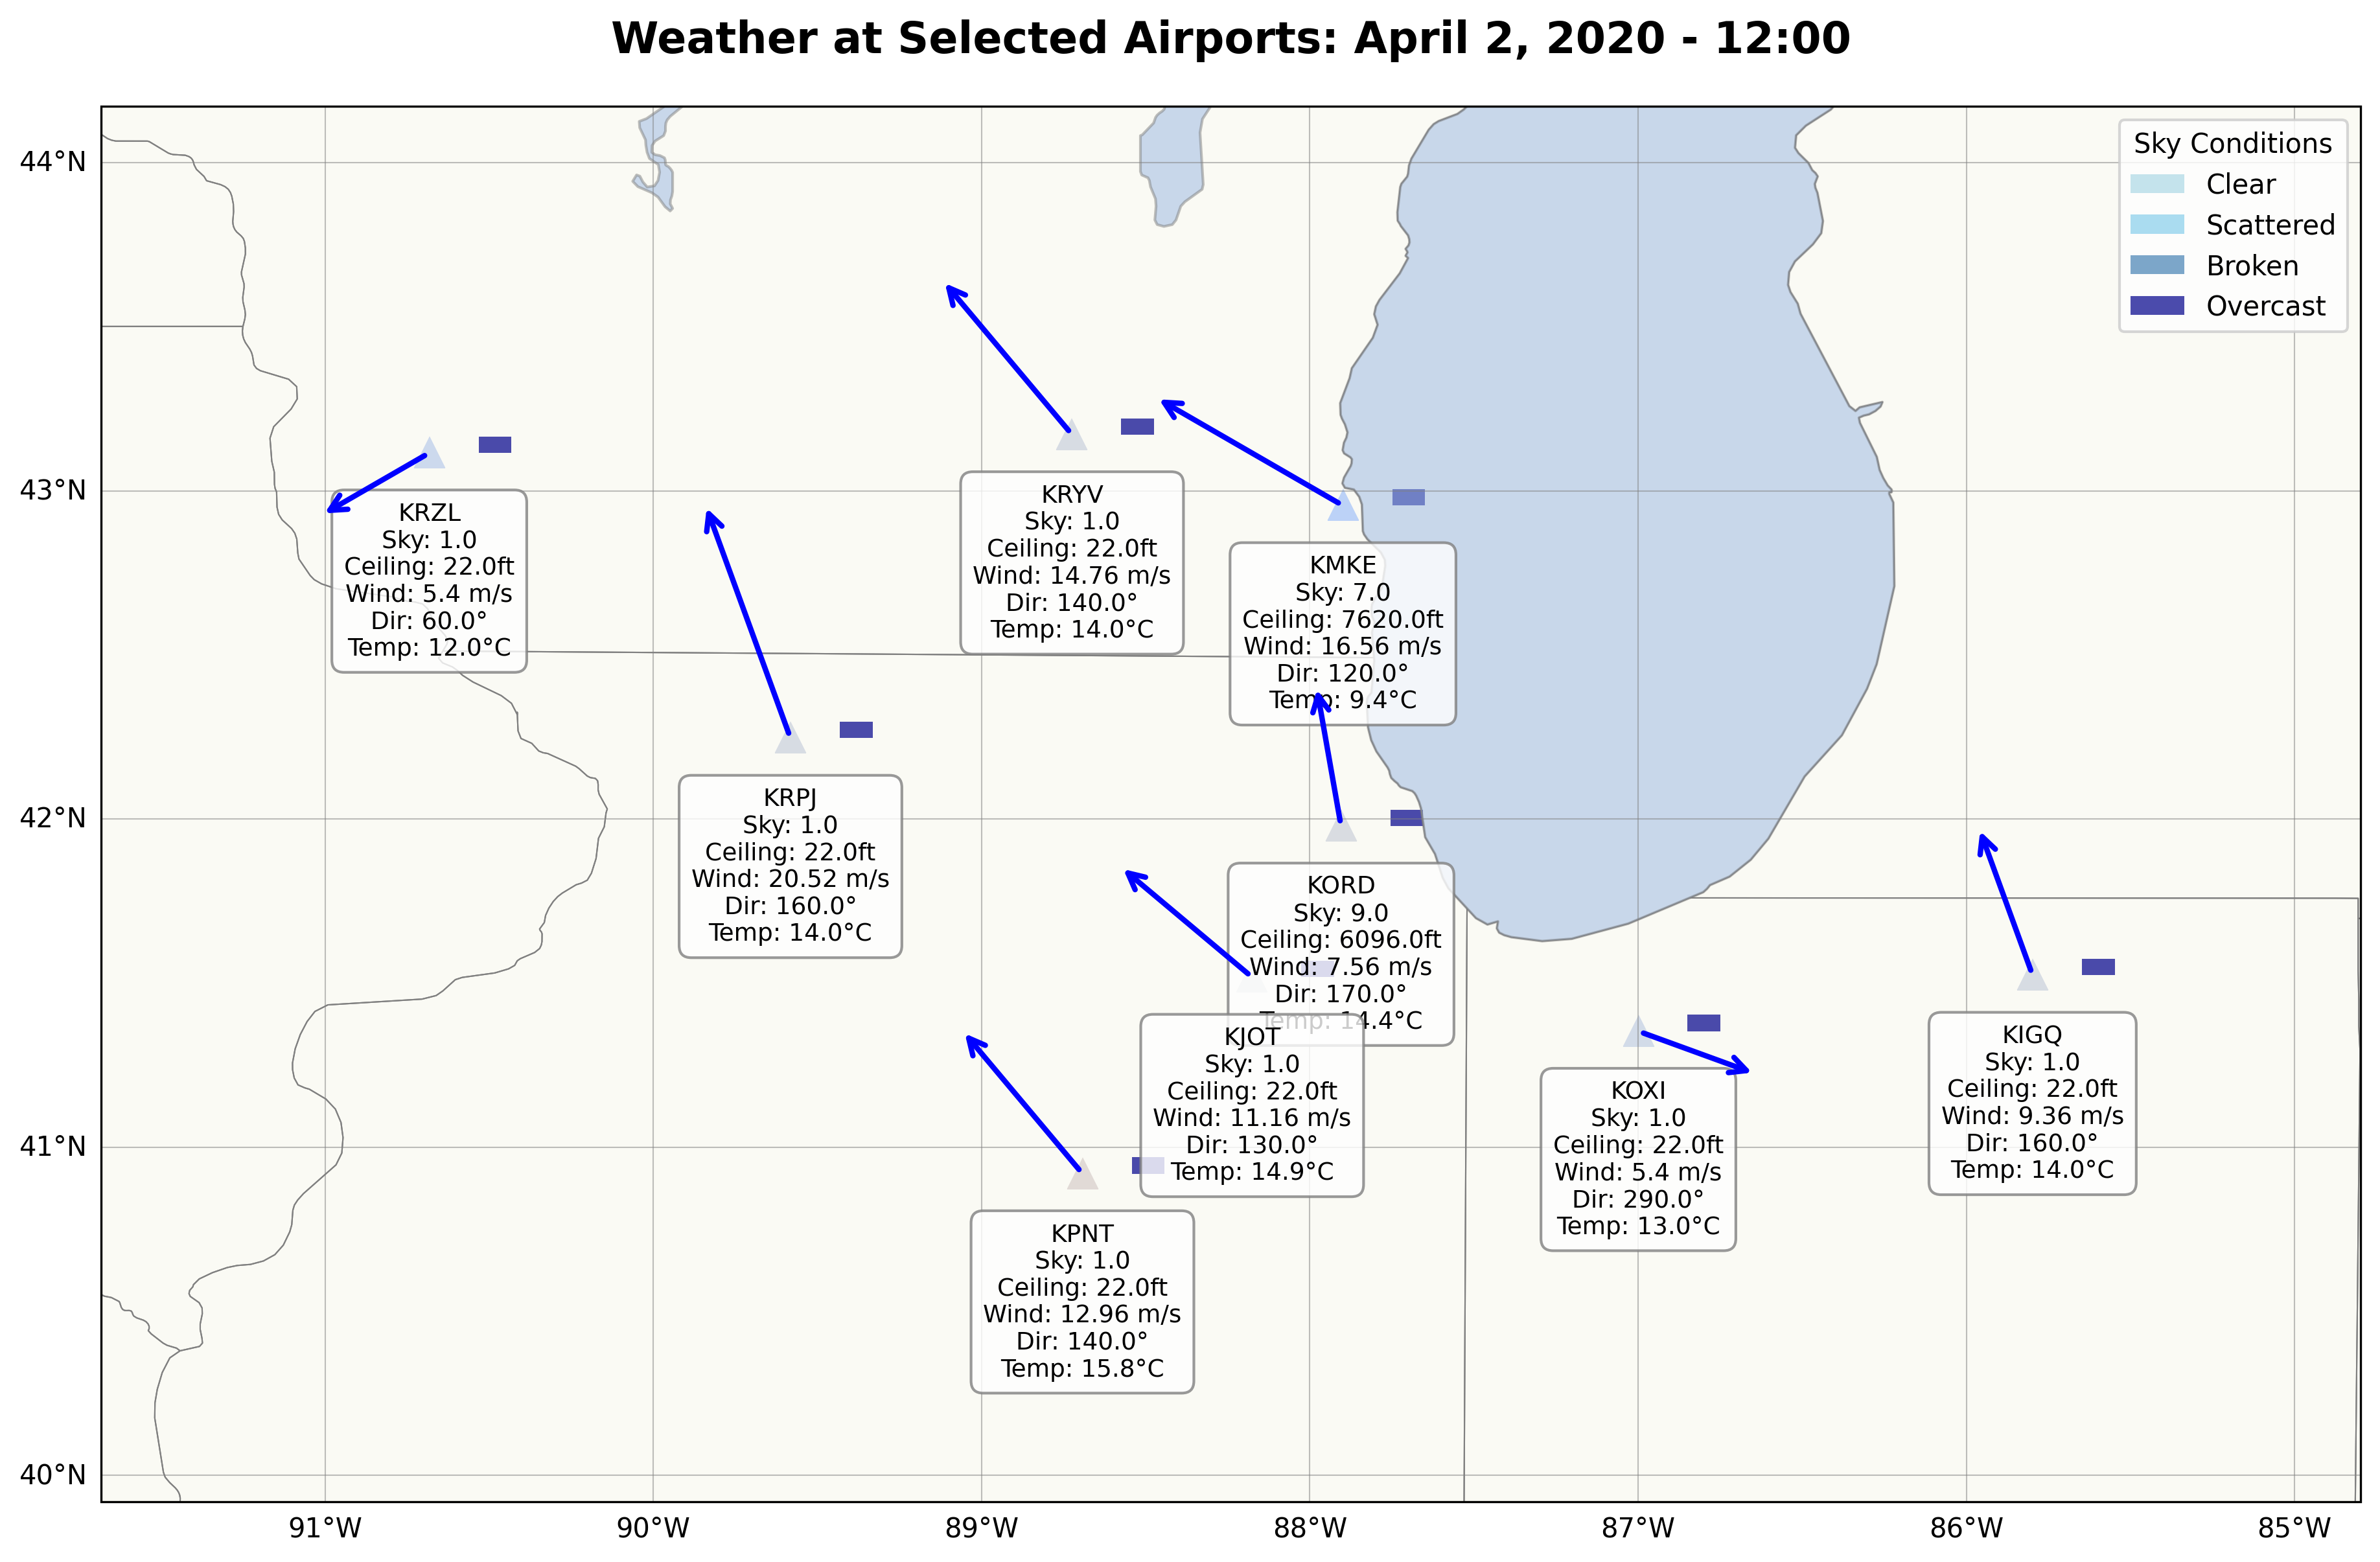
\includegraphics[width=\textwidth]{weather_map_12_00.png}
    \caption{Weather at Selected Airports: April 2, 2020 - 12:00}
    \label{fig:weather_12_00}
\end{figure}

\begin{figure}[H]
    \centering
    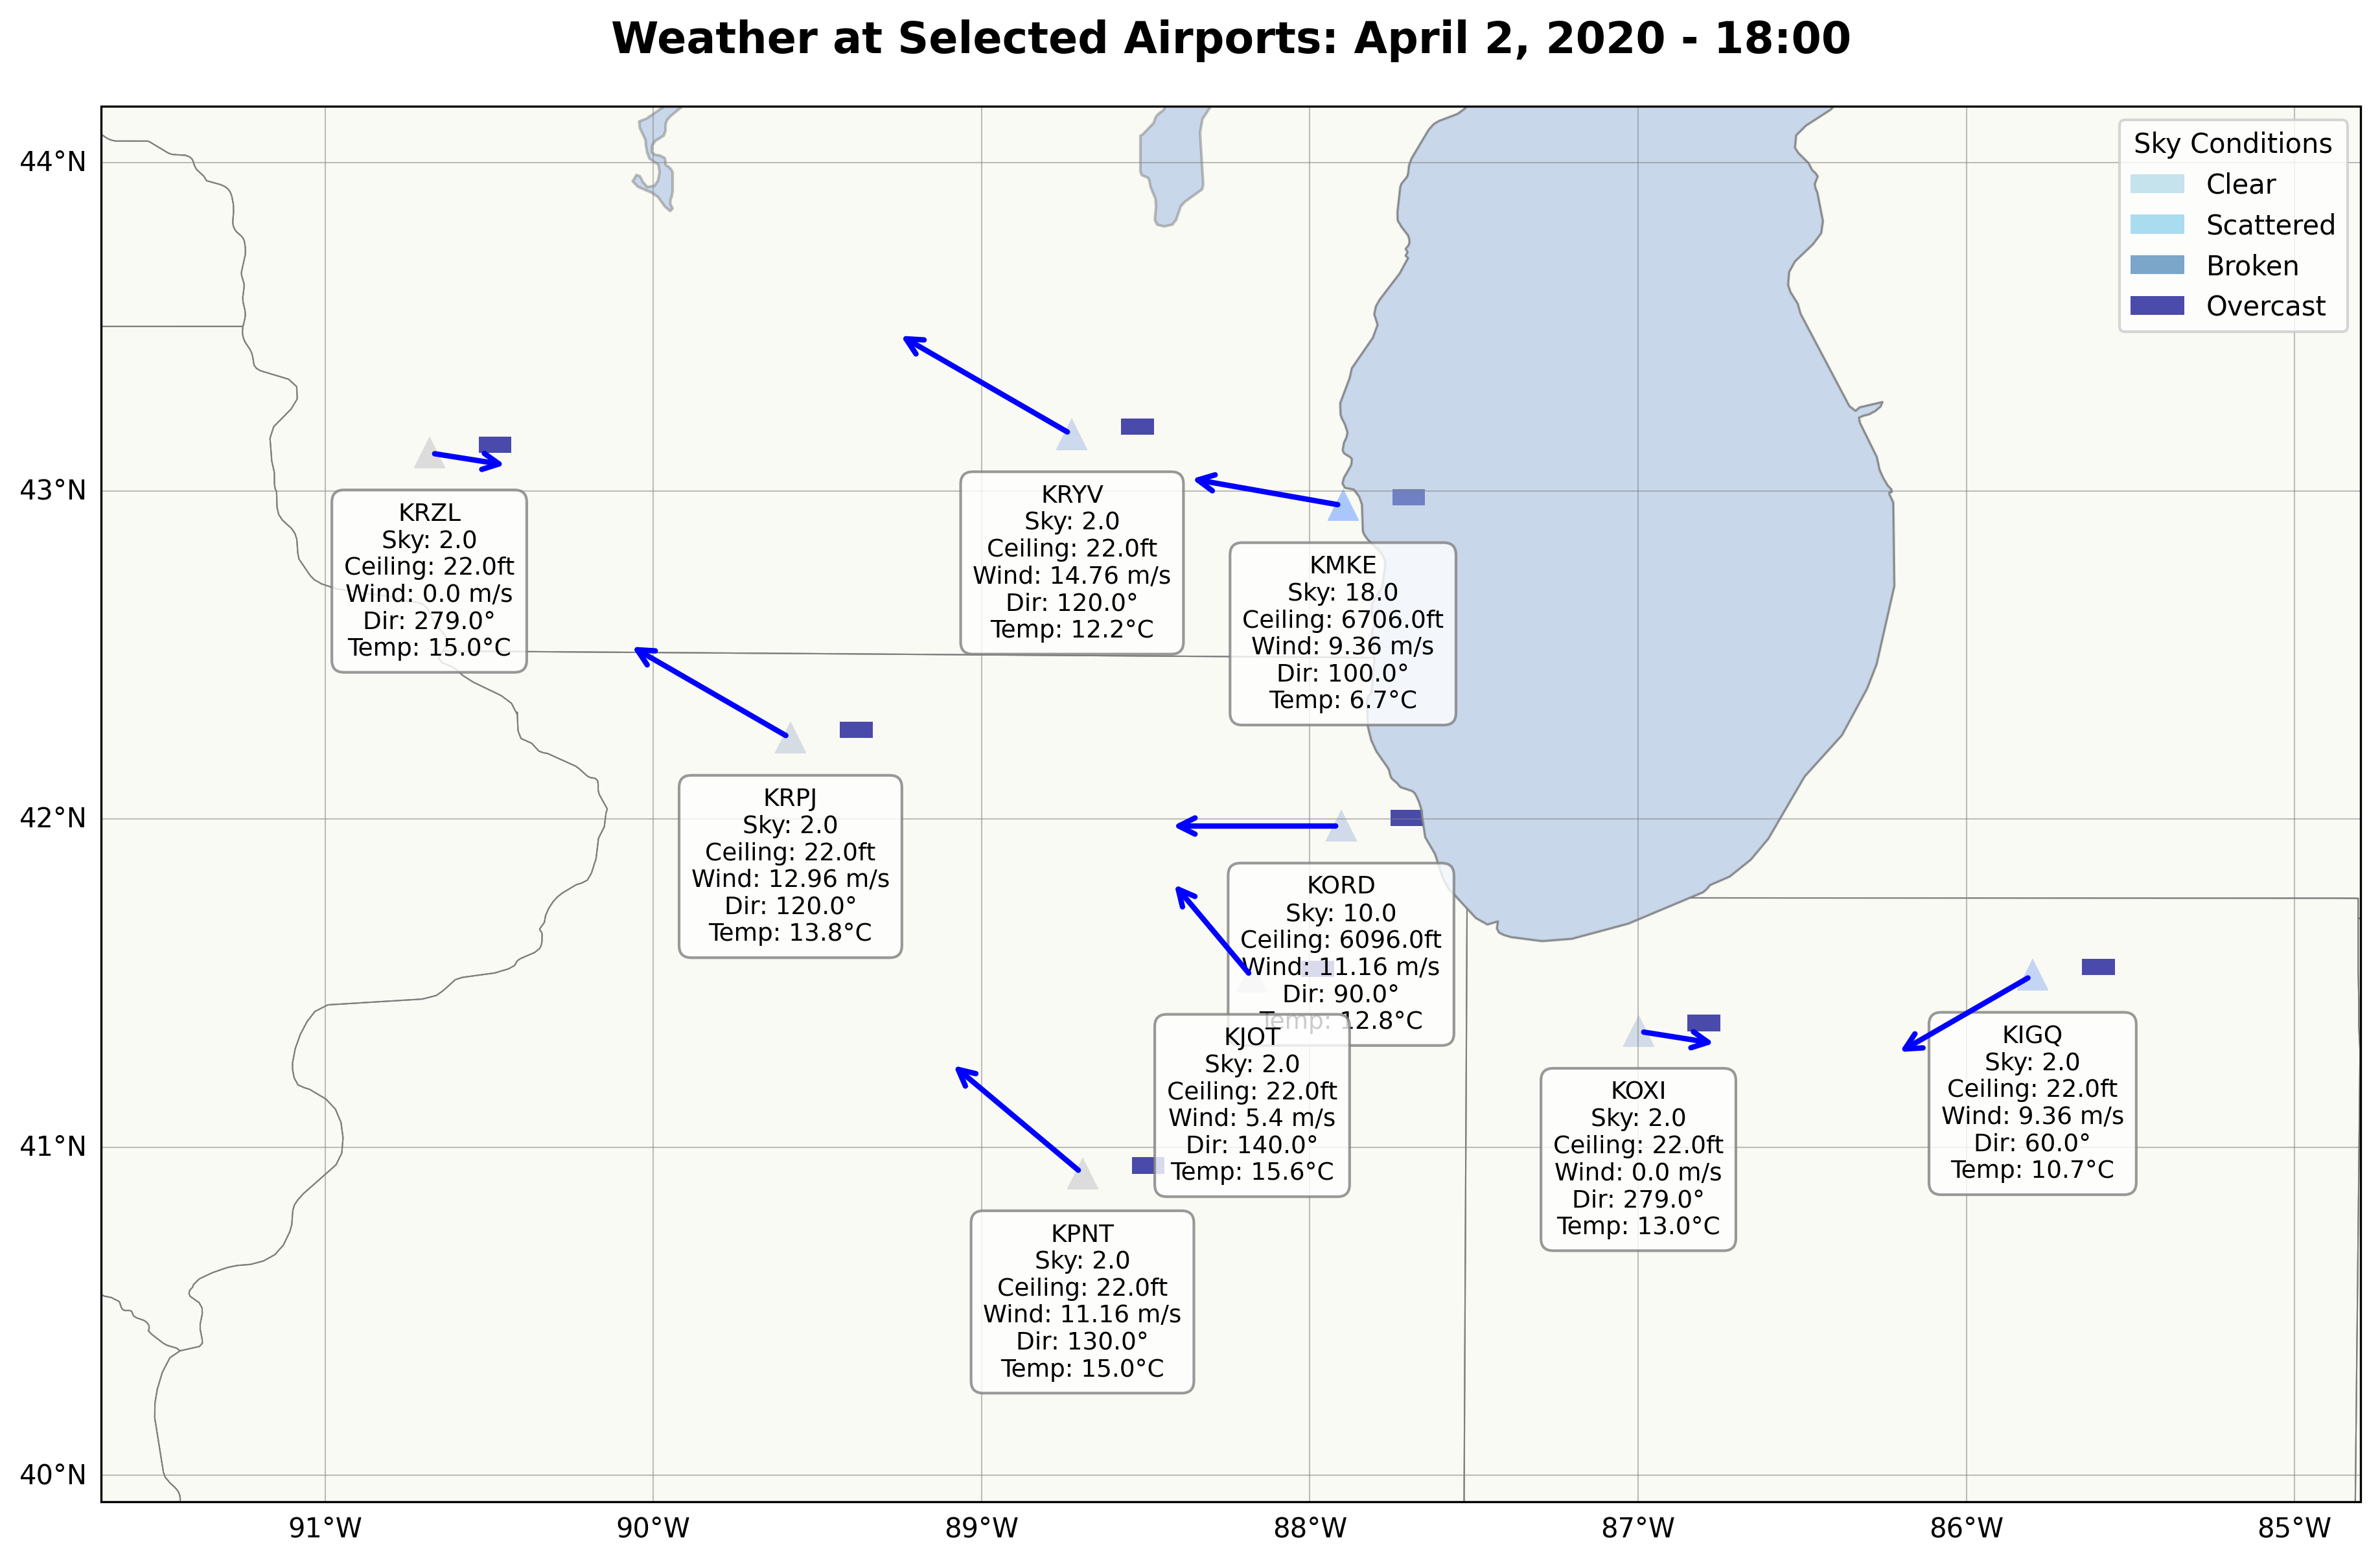
\includegraphics[width=\textwidth]{weather_map_18_00.png}
    \caption{Weather at Selected Airports: April 2, 2020 - 18:00}
    \label{fig:weather_18_00}
\end{figure}

\section{Weather Pattern Analysis}
These maps show how weather conditions evolved throughout April 2, 2020, across the Chicago metropolitan area and surrounding regions. The progression from midnight to evening reveals:
\begin{itemize}
    \item Daily temperature variations
    \item Wind pattern changes
    \item Cloud cover development
    \item Regional weather system movements
\end{itemize}

\end{document}
